\documentclass[journal]{IEEEtran}
%\usepackage[spanish]{babel}
\usepackage[utf8]{inputenc}
\usepackage{graphicx}
\graphicspath{ {images/} }
%\usepackage{enumerate}
\usepackage{amsmath}
\usepackage{mathtools}
\usepackage{float}
\usepackage{amssymb}
\usepackage{listings}
%\usepackage{caption}
\renewcommand{\IEEEkeywordsname}{Keywords}

\bgroup
\def\arraystretch{1.5}


\lstset{
basicstyle=\footnotesize
%,
%numbers=left
}

\begin{document}

\title{\textbf{Lab1: Power in home appliances}}
\author{
  \IEEEauthorblockN{ Jorge Lambra\~no$^3$, Julian Rojas$^2$, 
  Juan Sánchez$^3$\vspace{0.2cm}}\\
  \IEEEauthorblockA{\texttt{\small{$^1$jelambrano, $^2$drojasj,
   $^3$paradac @uninorte.edu.co
   }}}
}

\markboth{Lab1: Power in home appliances}%
{Shell \MakeLowercase{\textit{et al.}}: Bare Demo of IEEEtran.cls 
for Journals}
	
\maketitle

\begin{abstract}
This report presents the design and implementation 
of a security box and a dimmer circuit using DIACs 
and TRIACs. The reader also can find  the validation 
review with the theoretical model seen in class.    
\end{abstract}

%-----------------------------------------------------------

\begin{IEEEkeywords}  
Current, Power, Power Factor, Voltage, Waveform.
\end{IEEEkeywords}

%-----------------------------------------------------------
\IEEEpeerreviewmaketitle
%--------------------------------------------------------------------------

\section{INTRODUCTION}

The main purpose of this practice is to perform an 
analysis on the wave form and measurements of three 
different type of load. Inside the security box there 
is a fuse to protect the equipment from any shortcut. 
We used a shunt resistor of 1 $\Omega$ and 10 W to measure 
current dividing the voltage by 1 to obtain the actual 
current value. All electronics devices are composed of
resistances, capacitors and inductances, a soldering iron 
is a resistive linear load, they require 
heat to work. The voltage measured would be the same 
as the source but the current will vary depending on 
the power consumption of the device. We expect the same 
waveform for the voltage and current and no 
phase shift between them.\\

A drill would be an inductive linear load, based on 
the fact that motors are made of inductive coils. 
It should be a phase shift between voltage and current. 
The laptop is a nonlinear load, the voltage waveform 
would be the same but we expect a different shape for the 
current \textsuperscript{[1]}. \\

The second part consists on designing and developing 
an AC controller made of DIACs and TRIACs. This kind 
of circuit is able to change the RMS voltage on the 
terminals of a linear load by manipulating the 
firing angle of the TRIAC using a potentiometer. 
The load will not be linear anymore because of the 
electronic circuit resultant of the 
resistive load in series with the AC controller.\\

%--------------------------------------------------------------------

\section{PROCEDURE AND RESULT ANALYSIS}

\subsection{Power Computations}

The purpose of this practice is to measure the 
power consumption on electrical home devices, such 
as a laptop, a drill and a soldering iron. Taking into 
account that they work with high values of voltage 
and current compared with previous labs, precautions 
were taken in order to protect the devices and our 
integrity. The Figure \ref{circuit_diagram} 
shows the circuit proposed by the teacher to measure 
voltage and current safely. 

\begin{figure}[h]
\centering
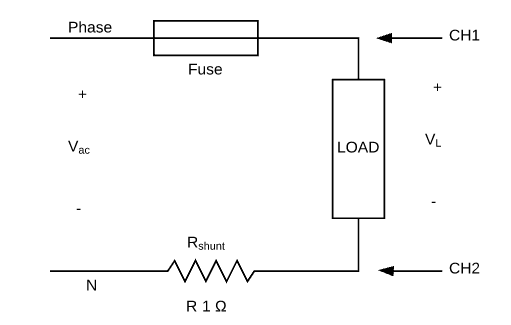
\includegraphics[clip,width=0.75\columnwidth]{circuit_diagram.png}
\caption{Circuit Diagram.}
\label{circuit_diagram}
\end{figure}

V\textsubscript{ac} represents the 120 Vrms sine wave 
obtained from the university phase line, \textit{Fuse}
represents a 3A circuit breaker, \textit{Load} represents 
the load and \textit{Rshunt} 
represents the 1 $\Omega$ and 10 W 
power resistor. We chose a small value for the resistor 
to do not affect the functioning of the circuit. \\

The gauge of the wire was selected depending on maximum 
current needed by the higher power load according to 
electrical parameters 
of each device. Current values of devices are 
shown on the Table \ref{current_table}. Based on this, 
AWG 14 wire was selected to build the power meter, because 
it is able to conduct a maximum of 15 A\textsubscript{rms}.
In addition to this, the circuit uses a 3A fuse to protect
load and wires of high currents.\\

\begin{table}
\centering
\caption{Power and current values of each device.}
\begin{tabular}{|l|p{1.2cm}|p{1.5cm}|p{1.5cm}|}
\hline 
Device & Power (W) & Voltage (V\textsubscript{rms}) 
& Current (A\textsubscript{rms}) \\ \hline 
Solderin Iron 	&  40	& 120 	& 0.33 \\ \hline 
Drill 		& 130	& 120   & 1.08 \\ \hline 
Laptop 		& 140 	& 120   & 1.16 \\ \hline 
Light Bulb		& 70  	& 120   & 0.58 \\ \hline 
\end{tabular}
\label{current_table}
\end{table}

The circuit is inside a 4x4 box with a fuse holder to 
change the breaker, 4 measuring terminals; the white 
one for neutral, green one for ground and 
both black one for phase. The box is shown in the 
Figure \ref{circuit_box}. \\

\begin{figure}[h]
\centering
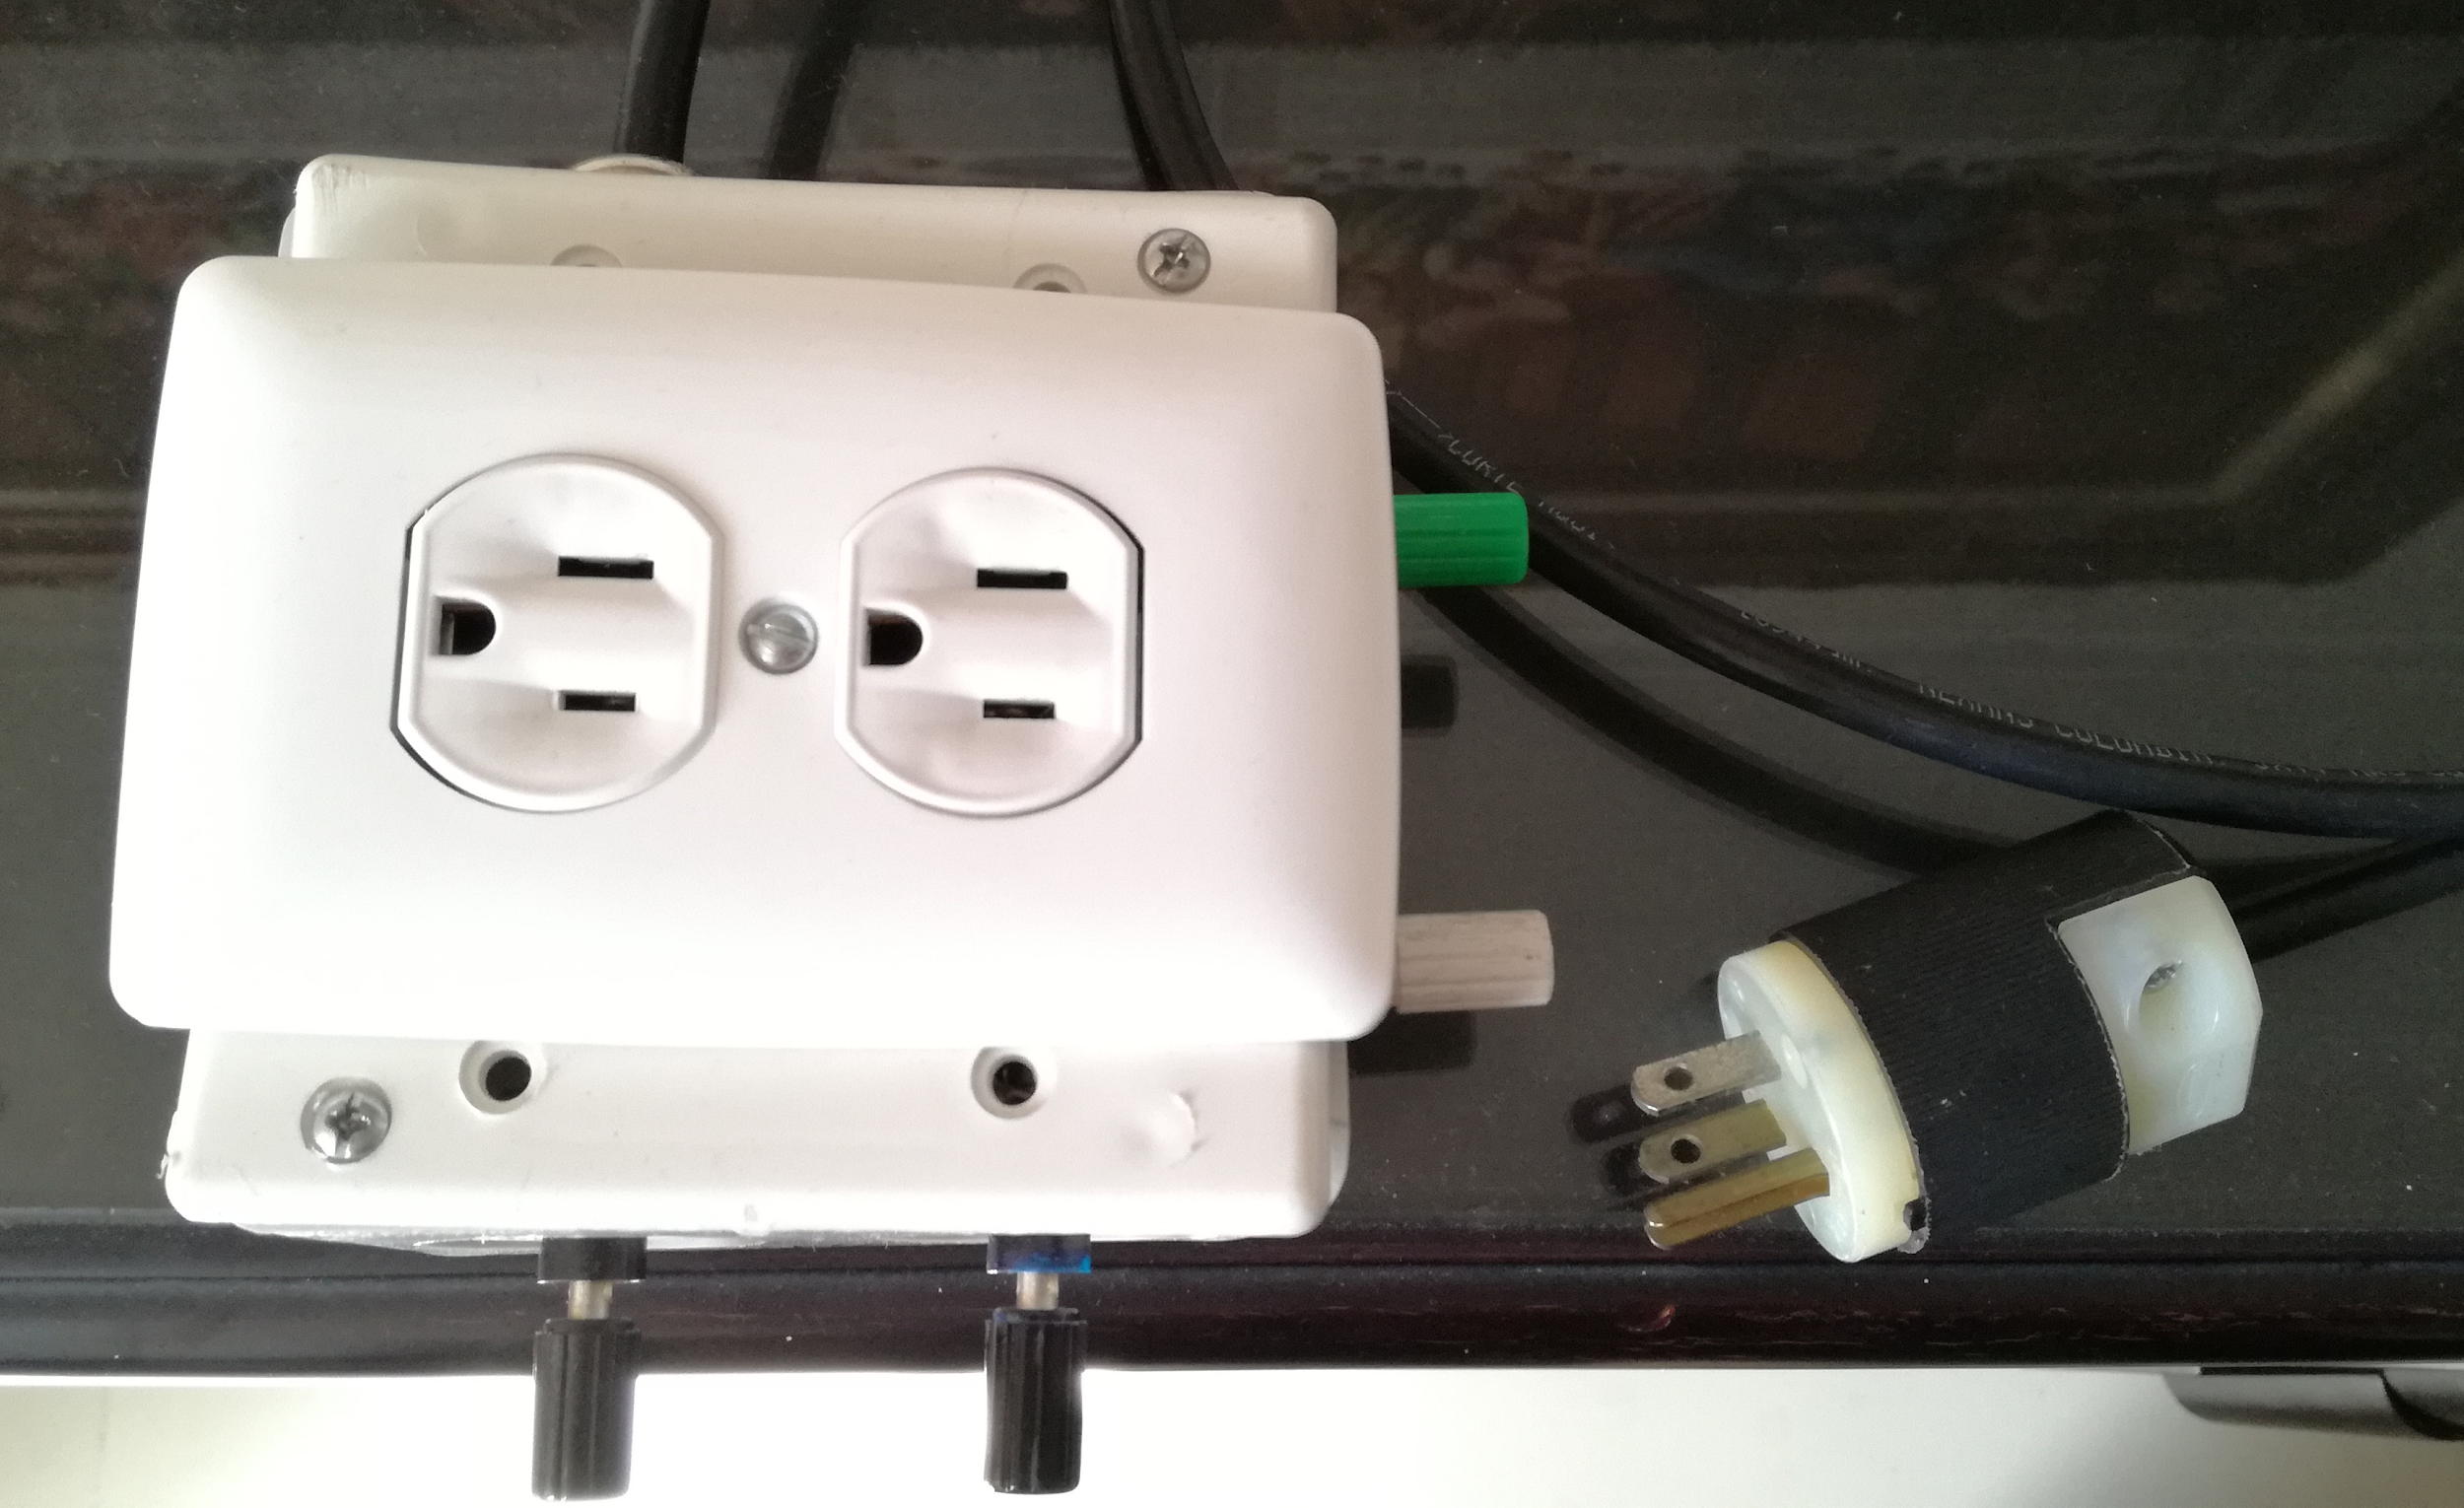
\includegraphics[clip,width=\columnwidth]{circuit_box.png}
\caption{Circuit box.}
\label{circuit_box}
\end{figure}

For this practice three different loads are chosen to 
analize their voltage and current waveform: 
a soldering iron 
like resistive load, a drill like inductive load and 
a laptop like non-linear load. These loads are conected 
to an electrical outlet, using the power meter. Owing to 
high electrical network inertia, the voltage waveform do
not depend on the load. For this reason, the voltage signal
is similar in all measurings. However, current waveform 
depend on impedance load and voltage, and the first 
parameter is realted to load features. Therefore, the 
power analysis will be centered on current waveform.\\

\subsubsection{Solderin Iron (resistive load)}
The current waveform is a pure sine signal and it does not 
present any distortion and between voltage and current there
are not phase difference. This can be observed in the Figure
\ref{original_resistive_load}. 

\begin{figure}[h]
\centering
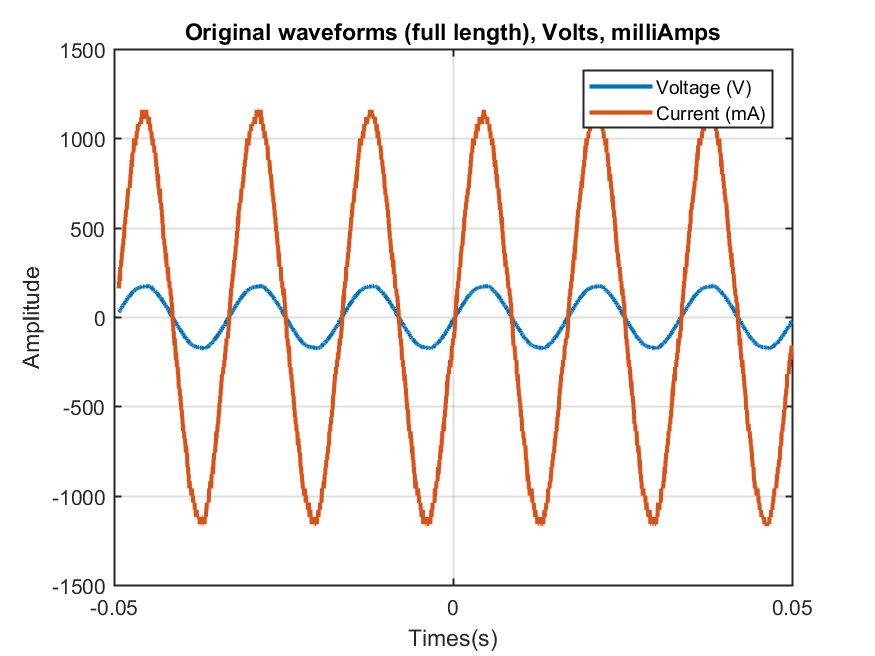
\includegraphics[clip,width=\columnwidth]{original_waveform_cautin.png}
\caption{Voltage and current waveforms of a resistive load.}
\label{original_resistive_load}
\end{figure}

Additionally, in a resistive load, product between 
current and voltage always 
is positive, this means that soldering iron is a power 
consumer and it is not able to supply energy. 

\begin{figure}[h]
\centering
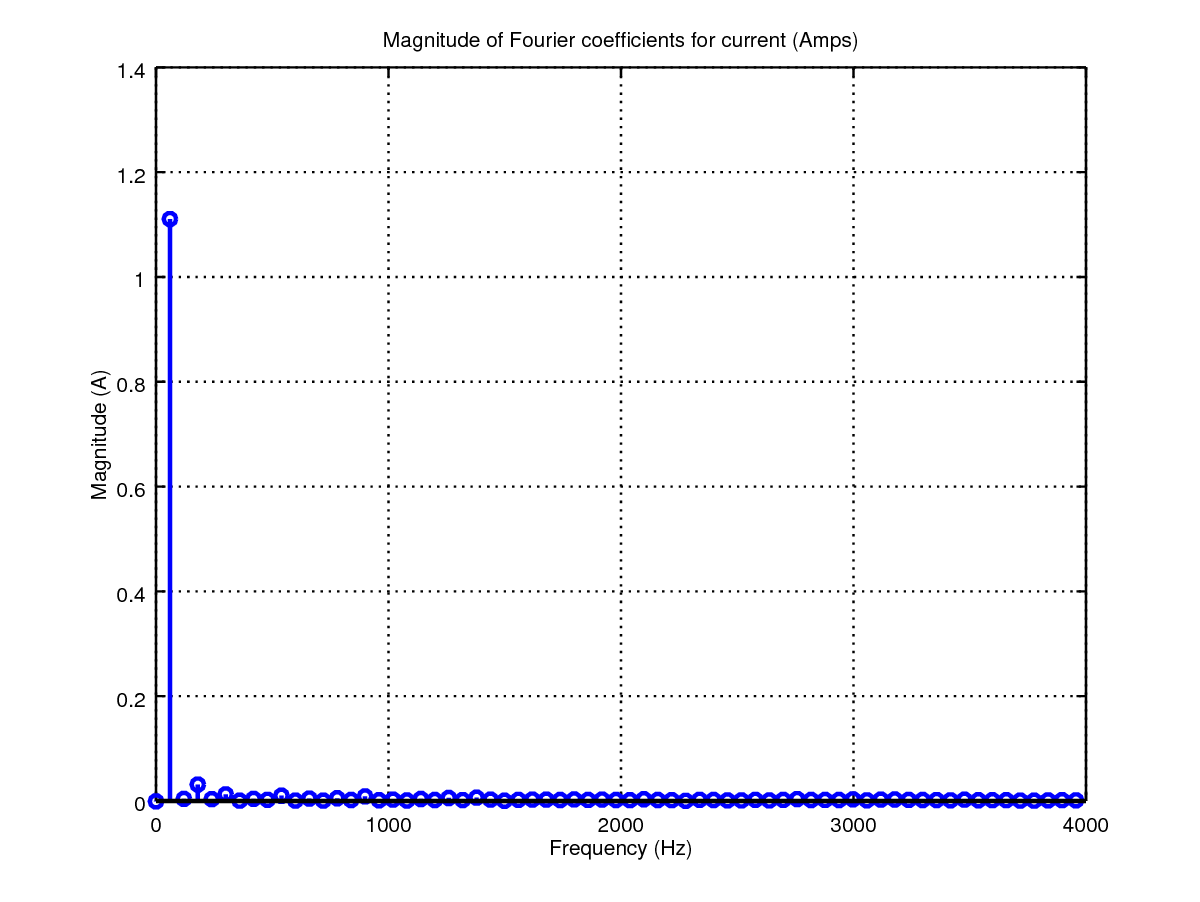
\includegraphics[clip,width=\columnwidth]
{zoomed_current_furier_coefficients_resistive.png}
\caption{Furier current coefficients for resistive load.}
\label{fourier_corrent_coefficients_resistive}
\end{figure}

Furier Transform allow to identify harmonic components of
current signal. According to Figure
\ref{fourier_corrent_coefficients_resistive}, current 
waveform of a resistive load only have a 60 Hz component
and it does not have any different harmonic component. So, 
there are not distortion, the power factor \textit{PF} is 
high and Total Harmonic Distortion \textit{THD} is 
very small.
This is an important feature from resistive loads.  

\begin{lstlisting}[caption = Output for resistive load.]
T     =     0.0167 s 
f0    =    59.9520 Hz 
Vrms  =   123.3322 V
Irms  =     0.7860 A
S     =    96.9336 VA
Pavg  =    96.8309 W 
P     =    96.8309 W 
Q     =    -1.8282 VAR 
D_fast=     4.0701 VA 
D     =     4.0562 VA 
PF    =     0.9989 
THD_V =     1.8878 %
THD_I =     4.0154 %
\end{lstlisting}

\subsubsection{Drill (inductive load)} The current 
behaviour for inductive loads is different to resistive 
loads. Current waveform is not a pure sine signal, 
because there are harmonic components that change shape 
current signal. This can be observed in the Figure 
\ref{original_inductive_load} and 
\ref{fourier_corrent_coefficients_inductive}. 
The waveform present peaks as a result of 
current harmonic component: $3 f_0$, $5 f_0$, $7 f_0$ 
and $9 f_0$,  where $f_0$ is fundamental frquency (60 Hz). 
In addition, there are an 
phase difference betweent both signal: current signal is
slow respect to voltage signal.

\begin{figure}[h]
\centering
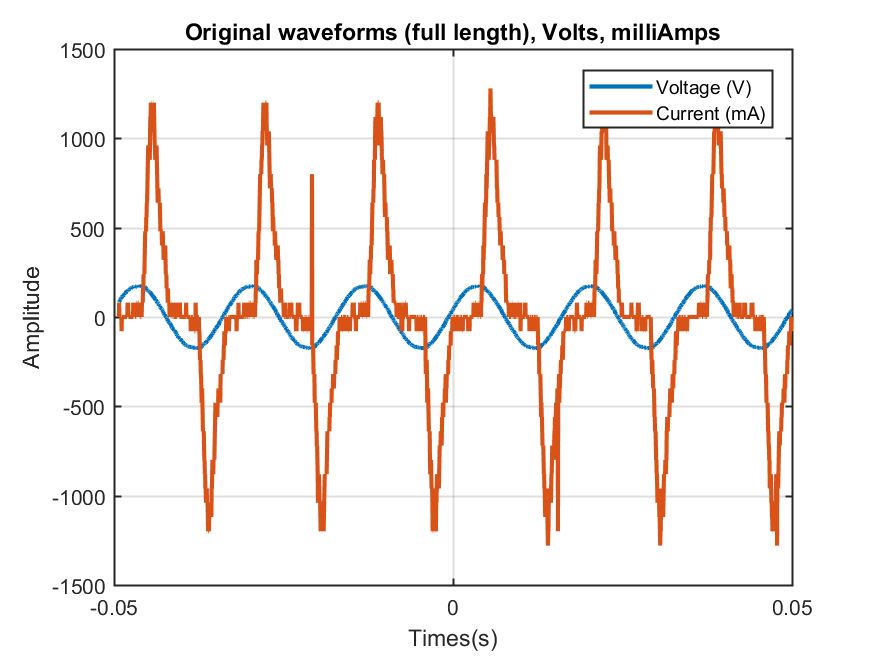
\includegraphics[clip,width=\columnwidth]
{original_waveform_drill.png}
\caption{Voltage and current waveforms of a inductive load.}
\label{original_inductive_load}
\end{figure}

In contrast to resistive load, the power factor value is 
very low and reactive power $Q$ and $THD_I$ are very high.
According to Listing \ref{output_inductive},
for this device, Reactive Power $Q$ is higher that Active 
Power $P$. 
This high $Q$ value mean that drill is a reactive element. 

\begin{figure}[h]
\centering
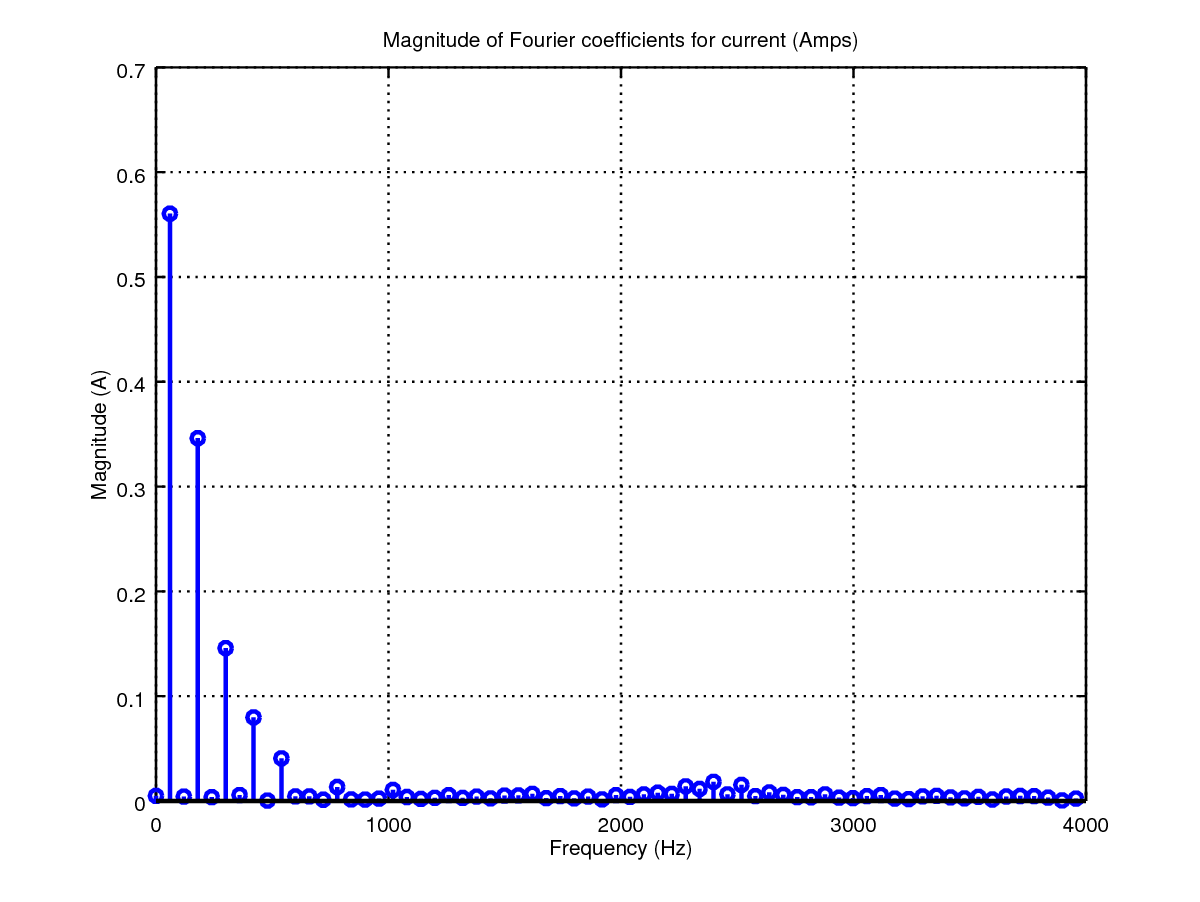
\includegraphics[clip,width=\columnwidth]
{zoomed_current_furier_coefficients_drill.png}
\caption{Furier current coefficients for inductive load.}
\label{fourier_corrent_coefficients_inductive}
\end{figure}

\begin{lstlisting} [caption = {Output for inductive load.}
\label{output_inductive}]
T     =     0.0167 s 
f0    =    59.9520 Hz 
Vrms  =   123.8850 V
Irms  =     0.4831 A
S     =    59.8537 VA
Pavg  =    30.4372 W 
P     =    30.4372 W 
Q     =    38.7767 VAR 
D_fast=    33.9472 VA 
D     =    33.9434 VA 
PF    =     0.5085 
THD_V =     1.8561 %
THD_I =    69.7550 %
\end{lstlisting}

\subsubsection{Laptop (non-linear load)} Finally, 
according to Figure \ref{original_no_lineal_load},  
current signal of non-linear load do not present any 
sine shape. The current waveform present peaks more 
narrow that inductive peaks loads. Those peaks 
presents a high harmonic components of current signal. 


\begin{figure}[h]
\centering
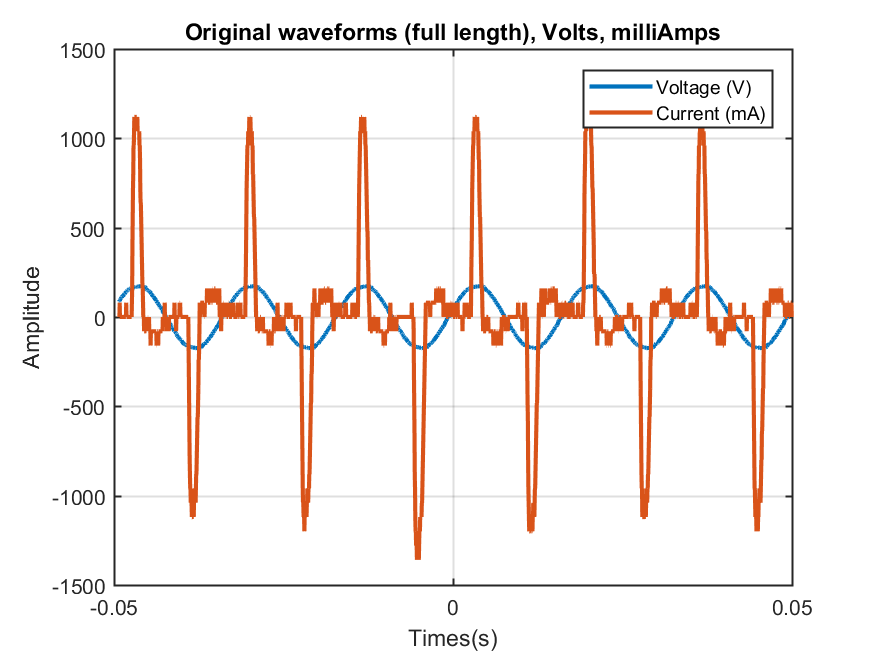
\includegraphics[clip,width=\columnwidth]
{original_waveform_computer.png}
\caption{Voltage and current waveforms of a non-linear load.}
\label{original_no_lineal_load}
\end{figure}

\begin{figure}[h]
\centering
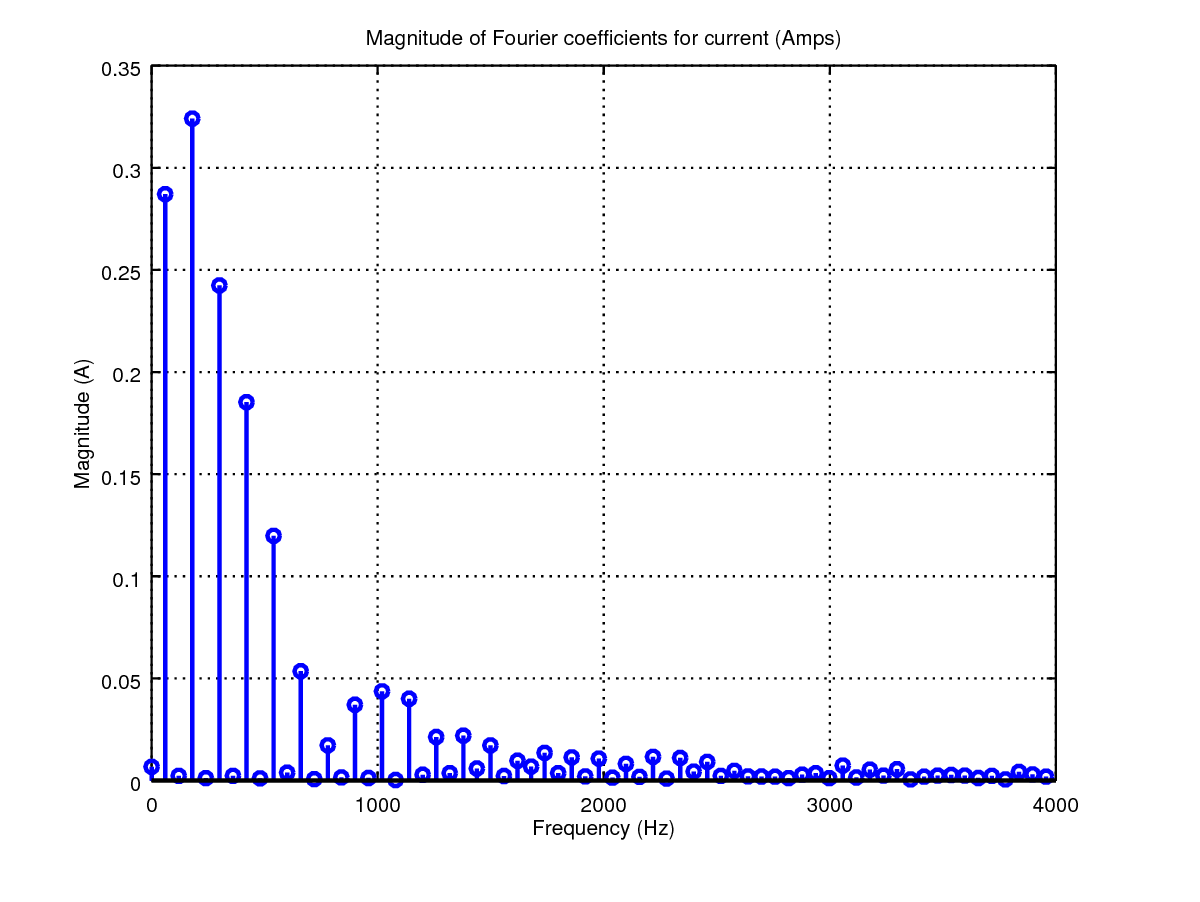
\includegraphics[clip,width=\columnwidth]
{zoomed_current_furier_coefficients_computer.png}
\caption{Furier current coefficients for non-linear load.}
\label{fourier_corrent_coefficients_nonlinear}
\end{figure}

\begin{lstlisting} [caption = Output for non-linear load.]
T     =     0.0167 s 
f0    =    59.9520 Hz 
Vrms  =   124.3447 V
Irms  =     0.3916 A
S     =    48.6915 VA
Pavg  =    23.9965 W 
P     =    23.9965 W 
Q     =    -5.7979 VAR 
D_fast=    41.9692 VA 
D     =    41.9644 VA 
PF    =     0.4928 
THD_V =     2.2668 %
THD_I =   164.9239 %
\end{lstlisting}

\subsection{AC contoller}

For the second part of the practice, a 
circuit using thyristors  was desinged to control 
the amount of power delivered to the light bulb. 
The input is the 120 V AC and 
the output is an AC waveform where there is a delay angle 
before triggering the AC voltage. The phase control is 
done with a potentiometer. The circuit designed is shown 
in the Figure \ref{ACcontroller}.

\begin{table}
\caption{Power measures from diferents controller values}
%elemento p q d fp th1
\begin{tabular}{|l|c|c|c|c|c|c|}
\hline 
Device & Active Power & Reactive Power & Harmonic Power & Aparent Power & Power Factor & THD \\ \hline
\end{tabular}
\end{table}

\begin{figure}[h]
\centering
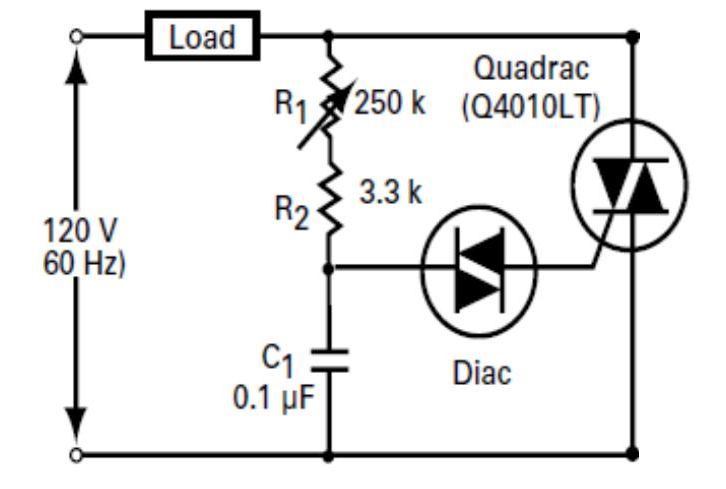
\includegraphics[clip,width=\columnwidth]{controller.png}
\caption{AC controller circuit.}
\label{ACcontroller}
\end{figure}

\section{CONCLUSIONS}

The resistive load shows a power factor of almost 1. 
The inductive load has a curly current shape, thanks to 
the type of motor being used in the drill. The 
non-linear load shows a kinky wave shape that 
depends on the circuit inside the electronic device.\\

Power computations let understand better the 
circuits, taking into account the meaning behind the 
power factor and the different kinds of 
power related to a circuit.\\

The dimmer allows to regulate the power taken by the 
light bulb. Taking into account that a light bulb is 
resistive, the effectiveness depends on the efficiency 
voltage and effective current. \\

The circuit is controlling the AC power to the light bulb 
by switching on and off during the positive and negative 
regions of the input sinusoidal signal. During the 
negative part of the input signal, the same type of 
response will be obtained since both the DIAC and TRIAC 
can be triggered in the reverse direction. Varying the 
resistance R, it is possible to control the driving 
angle. [3]\\

About inductive and non-linear loads, you shouldn't use 
the dimmer circuit, because both rely on the PF and the
voltage and current wave shape.\\

Electronic devices, such as,
DIACs and TRIACs let us build circuits to control the 
power taken by a resistive load.\\

\begin{thebibliography}{1}

\bibitem{IEEEhowto:kopka}
H.~Kopka and P.~W. Daly, \emph{A Guide to {\LaTeX}}, 3rd~ed.\hskip 1em plus
  0.5em minus 0.4em\relax Harlow, England: Addison-Wesley, 1999.

\end{thebibliography}

\end{document}